% !TEX root = ../../ThesisGchatzi.tex

\subsection{LS-Queries Using the \btsr}
\label{subsec:local_sim_search_methods}

\graphicspath{{Papers/SSTD2019/}{Papers/SIGSpatial2019/}}

A straightforward approach for answering LS-queries would be to use a spatial index to first filter by spatial distance and then perform a sequential scan across each result to filter out those having local similarity score below the given threshold. This suffers from generating an unnecessarily large number of intermediate results which are then discarded. Instead, we propose to process LS-queries by leveraging the \btsr index \cite{chatzig17btsr}, which can prune the search space simultaneously according to both criteria. 

While traversing the \btsr, {\em spatial filtering} is performed at each node $N$ by computing the {\em bounding distance} $mindist_{sp}$ between the location of $T_q$ and the MBR of $N$, as in R-Trees~\cite{DBLP:conf/sigmod/RoussopoulosKV95}.
  
For {\em time series similarity}, we exploit the MBTS stored within each node. Considering an MBTS $B$ at a node $N$, we calculate its distance $mindist_{ts}^i$ from $T_q$ at each timestamp $i$ as:
  
\begin{equation}
 \begin{split}
  mindist_{ts}^i(T_q, B_N) = \begin{cases}
    T_q.v_i - B_{N}^{\sqcap}.v_i, & \text{if} \;\; T_q.v_i > B_{N}^{\sqcap}.v_i \\
    B_{N}^{\sqcup}.v_i - T_q.v_i, & \text{if} \;\; T_q.v_i < B_{N}^{\sqcup}.v_i \\
    0, & \text{if} \;\; B_{N}^{\sqcap}.v_i \leq T_q.v_i \leq B_{N}^{\sqcup}.v_i
      \end{cases}
 \end{split}
 \label{eq:mindist_ts_local_sim}
\end{equation}

\noindent where $B_{N}^{\sqcap}.v_i$ and $B_{N}^{\sqcup}.v_i$ are the upper and lower values of the MBTS at timestamp $i$. By definition of MBTS, no time series indexed under $N$ can differ from $T_q$ by less than $mindist_{ts}^i$ at timestamp $i$. Hence, only at those timestamps that $mindist_{ts}^i \leq \epsilon$, it is possible that a time series indexed under $N$ is locally similar to $T_q$. Subsequently, we can compute a {\em local similarity bound} $\sigma_B$:
\begin{equation}
\sigma_{B}(T_q, B_N, \epsilon) = max\{|I|; \forall i \in I, mindist^i_{ts}(T_q, B_N) \leq \epsilon\}.
\label{eq:sim_bound}
\end{equation}
\noindent that reflects the {\em maximum} interval $I$ of consecutive timestamps where the distance computed by Eq.~\ref{eq:mindist_ts_local_sim} does not exceed margin $\epsilon$. 
This value is an upper bound of the local similarity scores of $T_q$ with any time series enclosed in this MBTS. Figure \ref{fig:sim_mbts} shows that $T_q$ deviates from the given MBTS by no more than $\epsilon$ during two intervals: one consisting of $|I_1|=5$ consecutive timestamps and a smaller one with only $|I_2|=2$ timestamps (shown as square points). So, the local similarity bound for this MBTS is $\sigma_{B}=5$.

\begin{figure}[!tb]
    \centering
    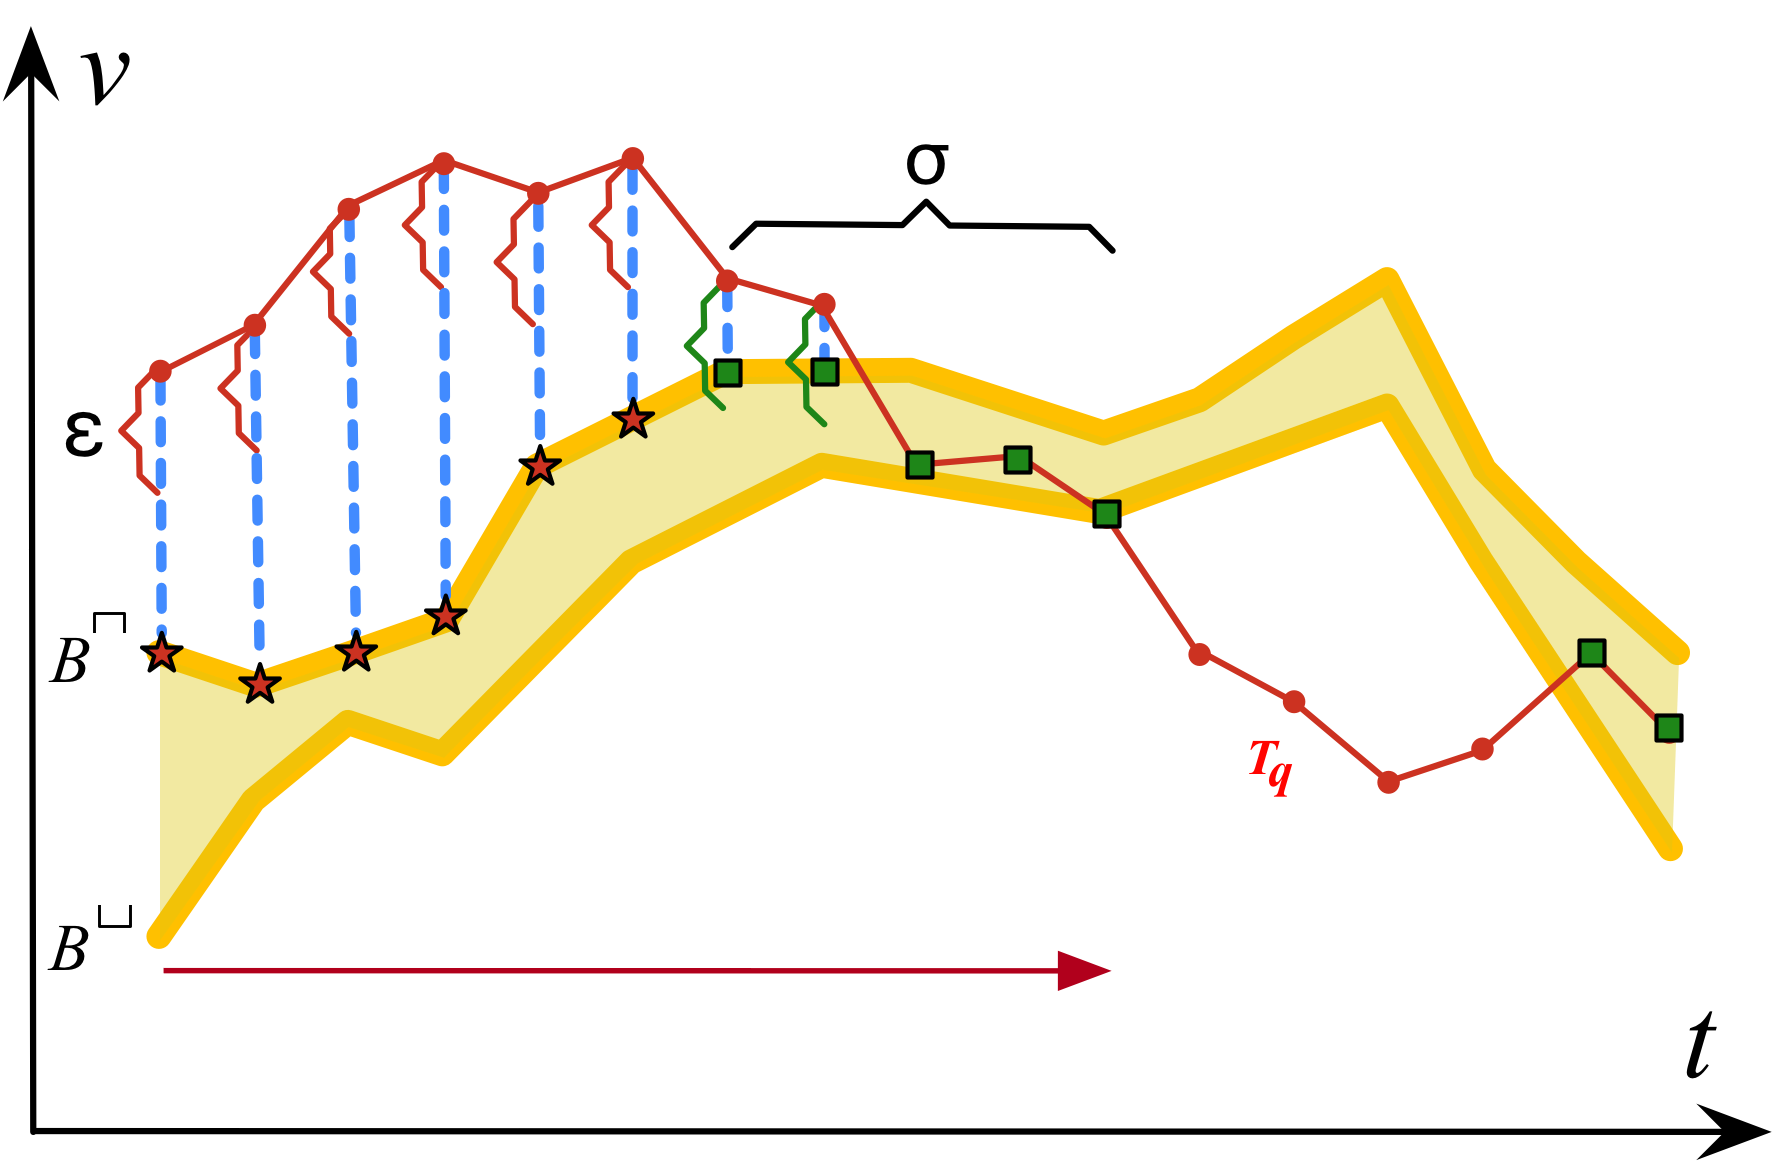
\includegraphics[width=0.5\textwidth]{Figures/sim_mbts.png}
    \caption{Local similarity check against an MBTS.}
    \label{fig:sim_mbts}
\end{figure}

By construction, the MBTSs of a child node $N'$ get tighter bounds compared to those of its parent $N$ as we descend the \btsr. It is easy to verify that 
\begin{equation}
\begin{split}
\sigma_{B}(T_q, B_N, \epsilon) \geq \sigma_{B}(T_q, B_{N'}, \epsilon)
\end{split}
\label{eq:maxdur_ts}
\end{equation}
\noindent hence local similarity bounds can only diminish when descending the index. This bound provides a useful pruning condition during search with a cutoff threshold $\delta$. Any node where all its MBTSs have local similarity bound $\sigma_{B}$ below $\delta$ can be safely pruned.

Next, we describe a baseline approach that employs a sequential scan over MBTSs, and then we present an optimization that prioritizes selected \textit{checkpoints} to avoid many point-wise comparisons.

\subsection{Sweep Line Approach}
\label{sec:baseline}

We explain how the \btsr can be used, in conjunction with a simple sweep-line algorithm, to answer each of the three LS-queries, taking advantage of the two types of bounds, $mindist_{sp}$ and $mindist_{ts}$, described above.

\noindent $\mathbold{Q_{rr}(T_q, \rho, \epsilon, \delta)}$: We traverse the \btsr starting from its root. At each inner node $N$, we first check whether $mindist_{sp}(T_q, MBR_N)$ $\leq$ $\rho$. If so, we employ a sweep line across the time axis to compute the local similarity bound $\sigma_{B}(T_q, B_N, \epsilon)$ for every MBTS included in $N$. If {\em all} resulting bounds $\sigma_{B}$ are below $\delta$, the subtree under $N$ is pruned. Otherwise, the search continues at the children. Upon reaching a leaf node, we fetch the geolocated time series contained therein, and verify the query constraints against each one. Each $T$ such that $dist_{sp}(T_q, T) \leq \rho$ and $\sigma(T_q, T, \epsilon) \geq \delta$ is added to the results.

\noindent $\mathbold{Q_{kr}(T_q, k, \epsilon, \delta)}$: We maintain a priority queue $P$ containing both inner nodes (sorted by ascending $mindist_{sp}$) and geolocated time series (sorted by ascending spatial distance to $T_q$). We start by adding to $P$ the root of \btsr. In each iteration, we retrieve the top element from $P$. If it is an inner node, we visit its children to calculate local similarity bounds $\sigma_B$ according to Eq.~\ref{eq:sim_bound}. For any child $N$ that $\sigma_B$ of one of its MBTSs satisfies threshold $\delta$, we search the subtree of $N$. Then, we calculate the corresponding spatial distance ($mindist_{sp}$ for a node $N$ or Euclidean distance for a geolocated time series $T$) and insert it back to $P$. Once we encounter a geolocated time series $T$ at the top of $P$, we add it to the results. The process terminates once $k$ geolocated time series have been obtained.

\noindent $\mathbold{Q_{rk}(T_q, \rho, \epsilon, k)}$: This query is evaluated similarly to the previous one, with two differences. The first difference is that the priority queue $P$ is now sorted based on local similarity bounds in descending order, instead of spatial distance bounds in ascending order. The second is that before inserting an item (node or time series) to $P$, its spatial distance ($mindist_{sp}$ or exact) is calculated, and if it is higher than $\rho$ the item is skipped. The traversal starts again from the root, and terminates once $k$ time series have been retrieved from the top of $P$. These are the top-$k$ results with respect to local similarity (if another time series $T$ had higher local similarity, it would have been retrieved from $P$ first), and they are located within range $\rho$ from $T_q$ (otherwise, they would not have been admitted to $P$). 

\subsubsection{Checkpoint Approach}
\label{sec:checkpoint_search}

The drawback of the sweep-line approach is that it needs to perform a comparison for each individual timestamp to eventually determine the exact or maximum local similarity of a given time series or node, respectively. In the following, we explain how we can use \textit{checkpoints} along the time axis to avoid this exhaustive search. These checkpoints prioritize specific timestamps when checking for candidate matches to eagerly filter out non-qualifying items.

Figure \ref{fig:checkpoints} shows an example with checkpoints placed along the time axis every $\delta=5$ timestamps. For clarity, we consider a single time series $T$. Assume a checkpoint at timestamp $t'$ and a minimal duration $\delta$ starting at timestamp $t'-\delta+1$ for asserting local similarity with query $T_q$, as shown with the grey strip in Figure \ref{fig:proof1}. This interval cannot have smaller duration, as it would not satisfy the $\delta$ constraint. Thus, the local similarity condition will evaluate to true at checkpoint $t'$. Similarly, if such an interval ends at timestamp $t'+\delta-1$ (Figure \ref{fig:proof2}), it will be detected at the checkpoint at $t'$. This observation entails that it suffices to check for local similarity only at checkpoints, i.e., every $\delta$ timestamps. We denote the set of checkpoints as $C$, determined at query time. If a checkpoint satisfies the condition, then we need to scan both forward and backward from it to determine the actual local similarity score, i.e., to find the exact extent of the time interval for which the condition holds.

Figure \ref{fig:sim_mbts_checkpoints} exemplifies the use of checkpoints for comparing $T_q$ to an MBTS of a node for $\delta=5$ timestamps. Instead of sequentially performing 11 comparisons until verifying that local similarity score $\sigma$ is at least $\delta$ (i.e., we stop the verification at $t=11$, once $\sigma=5$), we check only around the checkpoints. At the leftmost checkpoint $c_1$, no local similarity is found ($T_q$ is farther than $\epsilon$ from the MBTS), so we skip directly to checkpoint $c_2$. Since $T_q$ differs by less than $\epsilon$ at $c_2$, we need to compare values backward and forward, up to the previous and next checkpoint, respectively. This requires only 6 comparisons instead of 11 to decide that this node may contain candidates. Next, we describe how probing with checkpoints is applied during evaluation of LS-queries.

\begin{figure}[!tb]
    \centering
    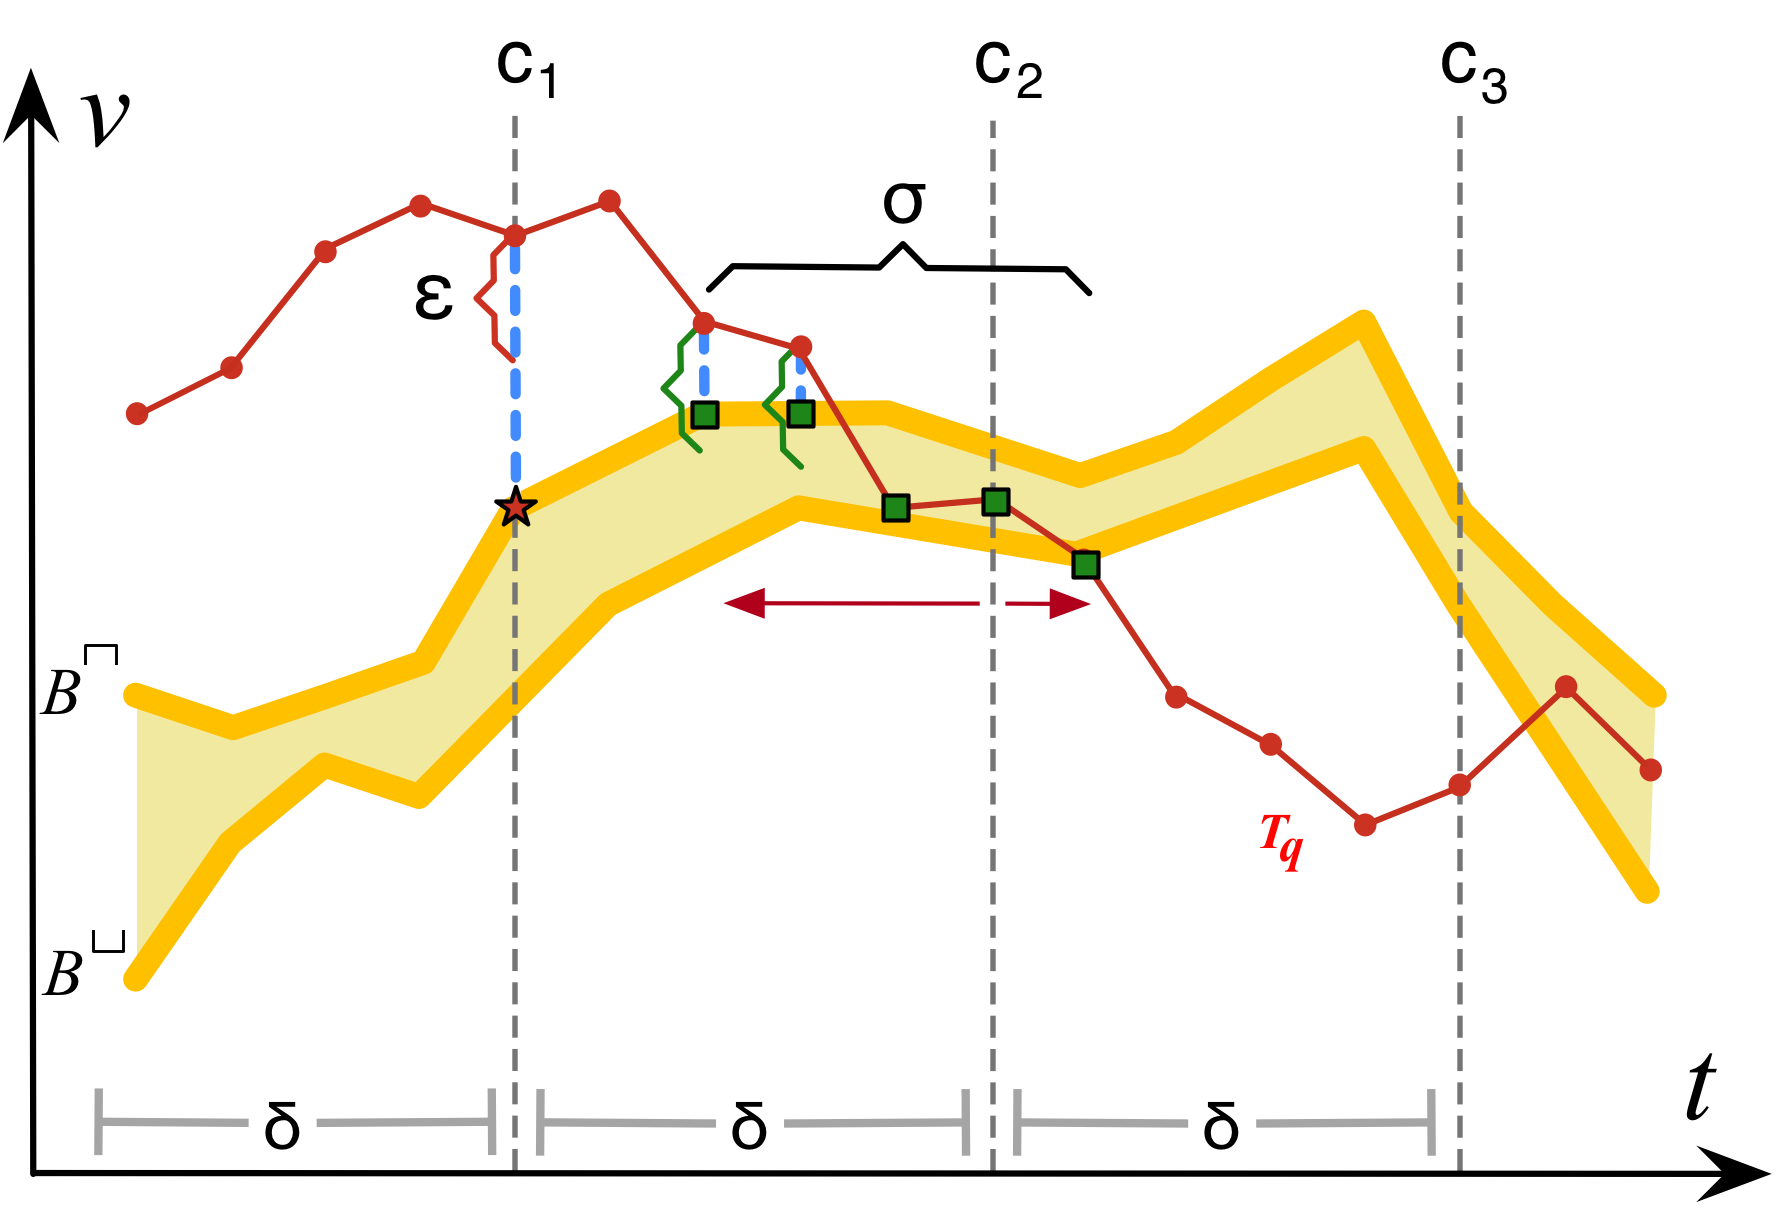
\includegraphics[width=0.5\textwidth]{Figures/sim_mbts_checkpoints.png}
    \caption{Local similarity with a MBTS using checkpoints.}
    \label{fig:sim_mbts_checkpoints}
\end{figure}

\noindent $\mathbold{Q_{rr}(T_q, \rho, \epsilon, \delta)}$: Algorithm \ref{alg:query_r} outlines the procedure. Initially, we obtain the children of the root node in a list and place the checkpoints every $\delta$ timestamps (Line 1). We iterate over each item $N$ in this list. If $N$ is an inner node, we have to examine whether both constraints with respect to $\rho$ and $\delta$ are met for each of its children. Verification of MBTS against query $T_q$ will be discussed shortly. If this is the case, we traverse the sub-tree of each child in the same manner, by adding it to the list (Lines 5-9), thus descending the tree. If the examined node is a leaf (Line 10), we iterate over each contained time series $T$ to check the constraints $\rho$ and $\delta$. If $T$ qualifies, it is added to the results (Lines 11-13). Note that now the calculation of local similarity scores for geolocated time series is based on checkpoints (Line 12), as discussed above.

Verification of MBTS against the local similarity constraints $\epsilon, \delta$ is applied using checkpoints (Lines~15-36). This verification concerns each MBTS in a given node $N'$. At each checkpoint $c$, we first verify whether its $mindist_{ts}^c$ to query $T_q$ is at most $\epsilon$ (Line 18). If so, we first scan backward to inspect whether there are at least $\delta$ consecutive timestamps where $T_q$ deviates by at most $\epsilon$ from this MBTS (Lines 20-27). Similarly, we probe forward from checkpoint $c$ (Lines 28-35). In either case, once local similarity no longer holds at a timestamp, probing skips to the next checkpoint. If the check fails for all checkpoints of all MBTSs, then this node cannot contain any results (Line 36).

\begin{algorithm}[!t]
    \DontPrintSemicolon
    \begin{footnotesize}
    \vspace{4pt}
    $R \leftarrow \emptyset, List \leftarrow Root.entries, C \leftarrow determineCheckpoints(\delta)$ \\
    \While{$List \neq \emptyset$}{
        $N \leftarrow List.getNext()$ \\
        \If{$N$ is not leaf}{
            \ForEach{$N' \in N.getChildren()$}{
                \If{$mindist_{sp}(T_q, MBR_{N'}) \leq \rho$}{
                    $count \leftarrow \emptyset$ \\
                    \If{$VerifyMBTS(T_q, N', C, \epsilon, \delta)$}{
                        $List \leftarrow List \cup \{N'.getChildren()\}$ \\
                    }
                }
            }
        }
        \Else{
            \ForEach{$T \in N.getObjects()$}{
                \If{$dist_{sp}(T_q, T) \leq \rho \land \sigma^C(T_q, T, \epsilon) \geq \delta$}{
                    $R \leftarrow R \cup \{ T \}$ \\
                }
            }
            \KwRet R
        }
    }
    
    \vspace{4pt}
    \SetKwProg{verifyMBTS}{Procedure}{}{}
    \verifyMBTS{$VerifyMBTS(T_q, N', C, \epsilon, \delta)$}{
        \ForEach{$B \in N'$}{
            \ForEach{$c \in C$}{
                \If{$mindist_{ts}^c(T_q, B) \leq \epsilon$}{
                    $count++, c' \leftarrow c$ \\
                    \While{True}{
                        $c'--$ \\
                        \If{$mindist_{ts}^{c'}(T_q, B) \leq \epsilon$}{
                            $count++$ \\
                            \If{$count \geq \delta$}{
                                \KwRet True
                            }
                        }
                        \Else{
                            $break$
                        }
                    }
                    \While{True}{
                        $c++$ \\
                        \If{$mindist_{ts}^c(T_q, B) \leq \epsilon$}{
                            $count++$ \\
                            \If{$count \geq \delta$}{
                                \KwRet True
                            }
                        }
                        \Else{
                            $break$
                        }
                    }
                } 
            }
        }
        \KwRet $False$
    }
    \end{footnotesize}
    \caption{$Q_{rr}(T_q, \rho, \epsilon, \delta)$}
    \label{alg:query_r}
\end{algorithm}

\noindent $\mathbold{Q_{kr}(T_q, k, \epsilon, \delta)}$: We follow a similar procedure to the one in Section~\ref{sec:baseline} for query $Q_{kr}$, employing the same verification process over MBTSs and time series as in Algorithm~\ref{alg:query_r}. Algorithm~\ref{alg:query_k} describes the procedure. We start by adding the root node to a priority queue $P$ based on spatial distance (Line 2). After determining the checkpoints using the given $\delta$ (Line 3), we iteratively retrieve elements from $P$ (Line 5). Then, three cases may occur: 
\begin{enumerate}
\item[(i)] If this element is a time series (Lines 6-9), it is guaranteed to be a result, given that $P$ is sorted based on spatial distance from $T_q$. Indeed, any subsequent element must be located farther than the current. When list $R$ obtains the required number $k$ of results, the search terminates. 
\item[(ii)] The element is a leaf node (Lines 10-14): In this case, we obtain each time series $T$ contained in this leaf, and verify the local similarity score of $T$ against $\delta$. If the condition is met, we calculate the spatial distance of candidate $T$ from query $T_q$ and push $T$ into the priority list along with its spatial distance (Lines 10-14). 
\item[(iii)] If the element is an inner node, we iterate over its children and only push back to the queue the ones whose MBTSs are verified against $\epsilon$ and $\delta$ using checkpoints (Lines 15-19).
\end{enumerate}

\begin{algorithm}[!t]
    \DontPrintSemicolon
    \begin{footnotesize}
    $R \leftarrow \emptyset$ \\
    $P.push(Root)$ \\
    $C \leftarrow determineCheckpoints(\delta)$ \\
    \While{$P$ is not empty}{
        $N \leftarrow P.poll()$ \\
        \If{$N$ is raw}{
                $R \leftarrow R \cup \{ N \}$ \\
            \If{$|R| = k$}{
                $break$ \\
            }
        }
        \ElseIf{$N$ is leaf}{
            \ForEach{$T \in N.getObjects()$}{
                \If{$\sigma^C(T_q, T, \epsilon) \geq \delta$}{
                     $T.dist \leftarrow dist_{sp}(T_q, T)$ \\
                     $P.push(T, T.dist)$ \\                  
                }                   
            }
        }
        \Else{
            \ForEach{$N' \in N.getChildren()$}{
                \If{$VerifyMBTS(T_q, N', C, \epsilon, \delta)$}{
                    $N'.dist \leftarrow mindist_{sp}(T_q, MBR_{N'})$ \\
                    $P.push(N', N'.dist)$ \\    
                }
            }
        }
    }
    \KwRet R
    \end{footnotesize}
    \caption{$Q_{kr}(T_q, k, \epsilon, \delta)$}
    \label{alg:query_k} 
\end{algorithm}

\noindent $\mathbold{Q_{rk}(T_q, \rho, \epsilon, k)}$: The procedure for this query is listed in Algorithm~\ref{alg:query_ks}. Notice that for employing checkpoints, we need a local similarity threshold $\delta$, so as to determine their placement, but this query does not specify a fixed $\delta$. To be able to obtain one during search, we now maintain two priority queues: $P$ holds inner nodes sorted by local similarity bounds (Eq.~\ref{eq:sim_bound}), while $R$ keeps up to $k$ geolocated time series sorted by local similarity scores (as in Def. 1). We initially set $\delta=1$, so checkpoints are trivially placed at every timestamp. This implies that computation of local similarity scores with $\delta=1$ is equivalent to the sweep line approach. However, $\delta$ increases with the detection of qualifying results, hence checkpoints will progressively get placed more sparsely. The search starts by adding the \btsr root in $P$ (Line 2). We iteratively poll the top element from $P$, and there are two possible cases:
\begin{enumerate}
\item[(i)] The top element is a leaf node. Then, we iterate over the contained time series and add the ones that satisfy the spatial condition ($\rho$) to $R$, along with their corresponding local similarity score $\sigma$ if it exceeds the current value of $\delta$ (Lines 8-12).
Once $R$ exceeds capacity $k$, its last element is evicted to make room for the newly inserted one and $\delta$ is updated according to the local similarity score $\sigma_k$ of the $k$-th element in $R$. In this case, the placement of checkpoints is re-adjusted according to the increased $\delta$ value (Lines 13-16).

\item[(ii)] The top element is an inner node. In this case, we iterate over each child $N'$ and check if $mindist_{sp}(T_q, {MBR_N'}) \leq \rho$. If $N'$ qualifies, we calculate the local similarity bound $\sigma_B$ of all its MBTSs using checkpoints. If the maximum among these bounds $max(\sigma_B) \geq \delta$, then $N'$ is inserted to $P$ with this maximum score (Lines 17-25).
\end{enumerate}

The process terminates once the top element in $P$ has local similarity less than $\delta$ (Lines 6-7). The result is the contents of $R$.

\begin{algorithm}[!t]
    \DontPrintSemicolon
    \begin{footnotesize}
    $R \leftarrow \emptyset$ \\
    $P.push(Root)$ \\
    $\delta \leftarrow 1$ \\
    $C \leftarrow determineCheckpoints(\delta)$ \\
    \While{$P$ is not empty}{
        \If{$P.peekFirst.\sigma_B < \delta$}{
            $break$ \\
        }
        \If{$N$ is leaf}{
            \ForEach{$T \in N.getObjects()$}{
                \If{$dist_{sp}(T_q, T) \leq \rho$}{
                     \If{$\sigma^C(T_q, T, \epsilon) \geq \delta$}{
                        $R.push(T, \sigma^C(T_q, T, \epsilon))$ \\                   
                     }
                }
                \If{$R.size > k$}{
                    $R.pollLast$ \\
                    $\delta \leftarrow R.peekLast.\sigma$ \\
                    $C \leftarrow determineCheckpoints(\delta)$ \\
                }
            }
        }
        \Else{
            \ForEach{$N' \in N.getChildren()$}{
                \If{$mindist_{sp}(T_q, MBR_{N'}) \leq \rho$}{
                    $\sigma_B \leftarrow 0$ \\
                    \ForEach{$B \in N'$}{
                        \If{$\sigma_B^C(T_q, B, \epsilon) \geq \sigma_B$}{
                            $\sigma_B \leftarrow \sigma_B^C(T_q, B, \epsilon)$
                        }
                    }
                    \If{$\sigma_B \geq \delta$}{
                        $P.push(N', \sigma_B)$ \\   
                    }
                }
            }
        }
    }
    \KwRet R
    \end{footnotesize}
    \caption{$Q_{rk}(T_q, k, \rho)$}
    \label{alg:query_ks}    
\end{algorithm}

\subsection{The \sbtsr Index}
\label{subsec:sbtsr_index}

\subsubsection{Index Structure}
\label{subsec:structure_sbtsr}
The \btsr index uses $k$-means clustering to cluster the time series under each node and then stores the MBTSs of those clusters. However, clustering entire time series typically generates many overlapping MBTSs, incurring much dead space. This has a negative impact on the pruning power of the index, especially when considering local similarities. Figure~\ref{subfig:bundles} depicts such a case of six time series indexed in a node. A $k$-means clustering with $k=3$ will form the depicted MBTSs denoted with shaded colors. As a result, the dark area $A$ represents the overlap between $mbts.1$ and $mbts.2$ and actually makes those bounds less tight. Hence, such MBTSs inflate estimates for local similarity bounds, and thus lead to unnecessarily descending further down the index.

To reduce the amount of overlap within the MBTSs of nodes, we introduce an extended version of the \btsr, named \sbtsr. \sbtsr attempts to eliminate as much overlap as possible, through segmentation of time series. Figure~\ref{subfig:bundles_part} depicts the intuition. If we segment the time series before applying $k$-means, the resulting MBTSs for each segment tend to be tighter, eliminating the excessive overlap $A$ from Figure~\ref{subfig:bundles}. The \sbtsr is built similarly to \btsr. The only difference is that the MBTSs of each node are calculated \textit{per segment}. In this method, we assume a pre-defined number $s$ of segments, but segmentation is orthogonal to our problem and can be carried out by applying existing methods like \cite{bingham2006segmentation}. Ultimately, \sbtsr allows for more aggressive pruning when traversing the index.

\begin{figure}[!tb]
 \centering
 \subfloat[Example of a node's MBTS.]{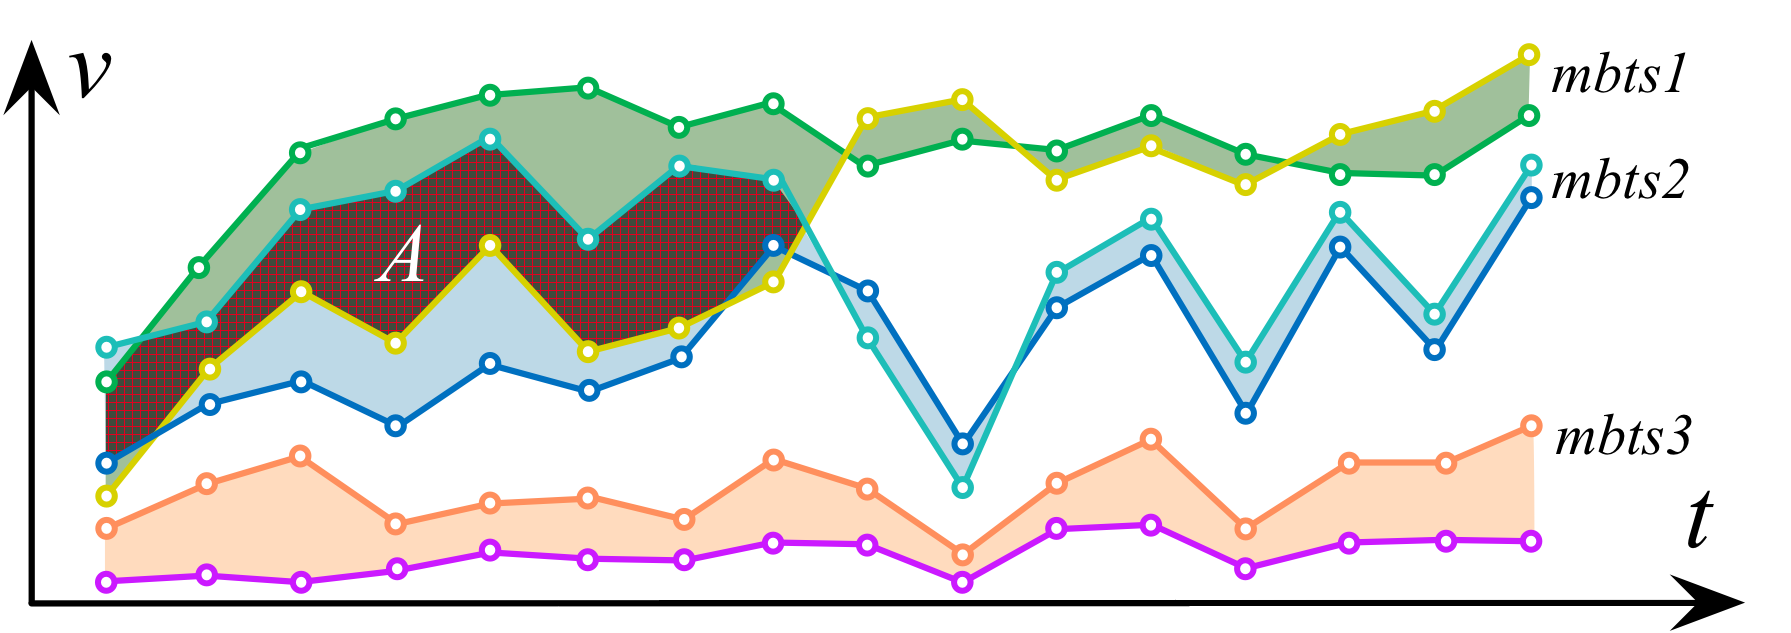
\includegraphics[width=0.6\textwidth]{Figures/bundles_node.png}\label{subfig:bundles}} \\
 \subfloat[Segmenting can eliminate whitespace.]{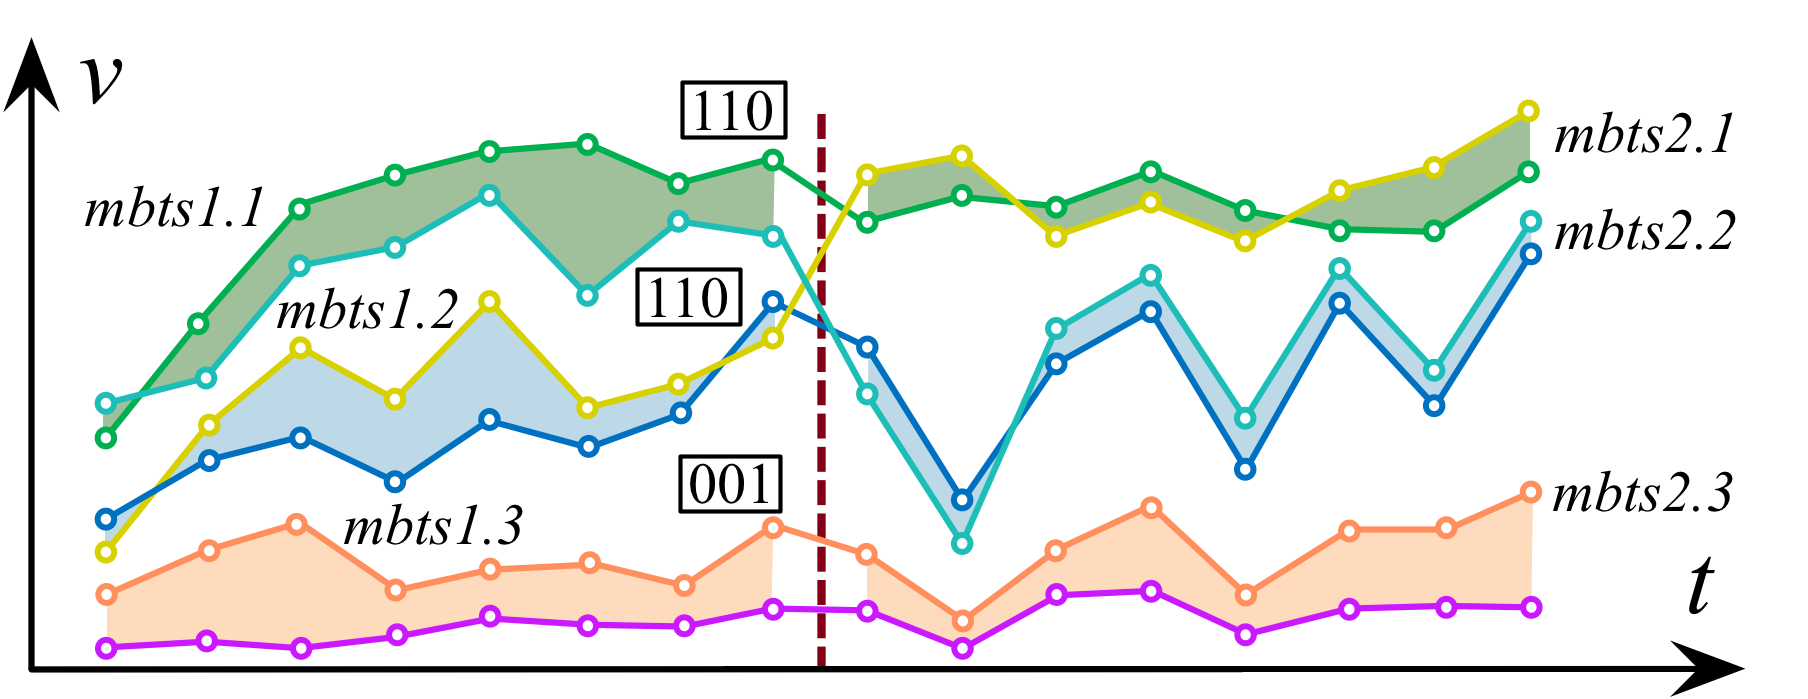
\includegraphics[width=0.6\textwidth]{Figures/bundles_node_partition.png}\label{subfig:bundles_part}}
 \vspace{-10pt} 
 \caption{Segmenting time series yields tighter MBTS.}
 \label{fig:proof_partition}
\end{figure}

\subsubsection{Cross-Segment Continuity Via Bit-Vectors}
\label{subsec:bit_vectors}
A downside of the segmentation approach is the loss of the MBTS continuity across time, which results in MBTSs enclosing different time series in neighboring segments. For example, in Figure~\ref{subfig:bundles_part}, there are no MBTSs in the right segment containing the same time series as $mbts1.1$ and $mbts1.2$, a fact which hinders the calculation of local similarity on the segment boundaries (the vertical line). To overcome this, we introduce a \textit{bit-vector} $V$ along each MBTS of a segment, having one bit for each MBTS created. If in the current segment a bit in vector $V$ of a given MBTS is set, this indicates that this MBTS encloses at least one common time series with another MBTS$'$ in the next segment. In the example shown in Figure~\ref{subfig:bundles_part}, $V=110$ for $mbts1.1$ indicates common time series with $mbts2.1$ and $mbts2.2$ in the next segment, while $V=001 $ for $mbts1.3$ signifies common time series with only $mbts2.3$. This way, to calculate local similarity, we can easily identify all the MBTSs that share common time series among two successive segments. 

To evaluate LS-queries, traversal of the \sbtsr index follows a similar rationale to the procedure in Section~\ref{sec:checkpoint_search}. For each checkpoint $c$, we first obtain the segment where it falls in, and we scan each MBTS leftward and rightward from $c$, as discussed in Section~\ref{sec:checkpoint_search}. If we cross the border to another segment, the available bit-vectors directly identify the MBTS that need be examined in this neighboring segment. This propagates until the local similarity constraints ($\epsilon$ and $\delta$) are satisfied. Figure~\ref{fig:part_checkpnt} illustrates an example of a node verification. Let us consider a predetermined number of three segments and the corresponding MBTS of each segment for that node. Suppose that there exists a checkpoint $c$ on the second segment. To verify whether this node satisfies the local similarity constraints, we start from checkpoint $c$ and we check leftwards whether $mindist_{ts}^{i} \leq \epsilon$ for each timestamp. If the currently examined timestamp falls in the first segment, we fetch the corresponding MBTS and bit-vectors and continue checking whether $mindist_{ts}^{i} \leq \epsilon$ in both MBTS (green shaded), as their bit-vectors both indicate common members with the first one in segment 2. A similar procedure is followed rightwards, where we only have to check the first MBTS, according to the bit-vectors.

\begin{figure}[!tb]
    \centering
    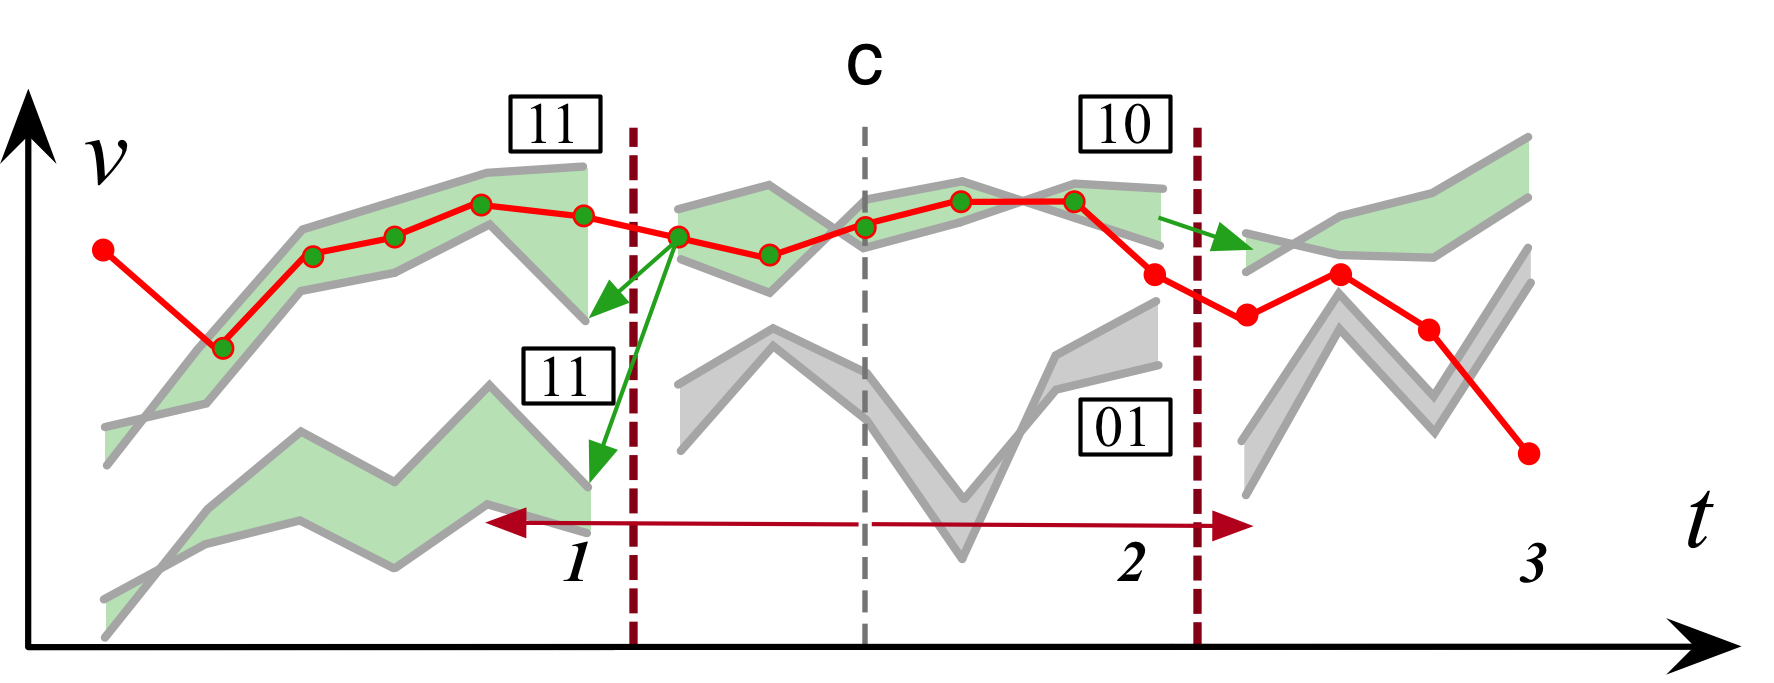
\includegraphics[width=0.6\textwidth]{Figures/partition_checkpoint_check.png}
    \caption{Example of verifying a \sbtsr node.}
    \label{fig:part_checkpnt}
\end{figure}

\subsubsection{Cost Analysis}
\label{subsubsec:cost}
Next, we analyze the cost of the $Q_{rr}$ query (the other queries have similar costs). For index traversal, since the index is an augmented R-tree, the basic cost for searching over an R-tree applies here as well~\cite{Guttman1984}. However, there is an extra cost which involves two parts. The first part concerns MBTS verification. Assume a query time series $T_q$ of length $n$ that is verified against the MBTS of a node $N$. For each checkpoint, the algorithm checks for each timestamp $t$ among two segments, whether the mindist at $t$ between $T_q$ and the node’s MBTS is less than $\epsilon$ (see Equation~\ref{eq:maxdur_ts}). This is repeated at each neighboring segment for each MBTS whose bit vector is $1$, until threshold $\delta$ is satisfied, or rejected for all checkpoints. Thus, this extra cost is $O(c*b^2*s*g)$ in the worst case, where $c$ is the number of checkpoints, $b$ is the number of MBTS, $s$ the number of segments, and $g=n/s$ the number of timestamps between two segments. In practice, this will typically require much fewer comparisons, since the node is traversed only when a qualifying interval is found. The second part of extra cost concerns time series verification. To verify $T_q$ against $T$, the algorithm needs to check for each timestamp $t$ whether the value difference between $T_q$ and $T$ is less than $\epsilon$, and keep the largest detected one; hence, this extra cost is $O(n)$.